\begin{wrapfigure}[17]{r}{0.5\linewidth}
\centering
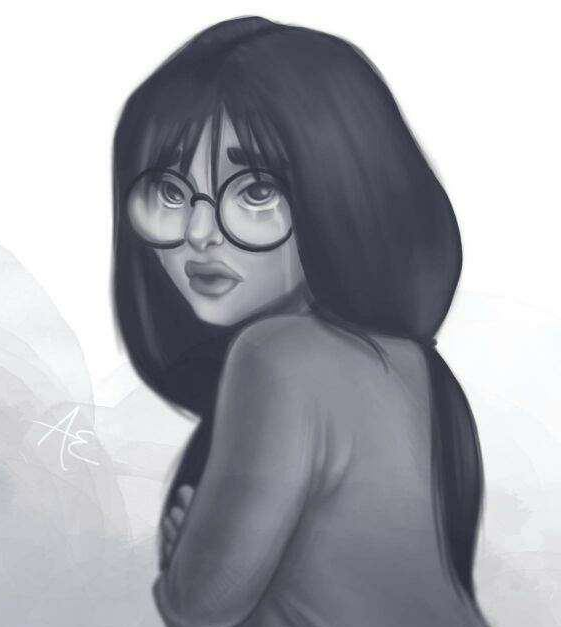
\includegraphics[max width=0.5\textwidth]{../Pictures/Characters/Portraits/Myrtle_portrait.png}
\end{wrapfigure}

\paragraph{Description}
Myrtle Elizabeth Warren is a brown-haired muggle-born witch. She is currently a student at Hogwarts and was sorted into the house of Ravenclaw because of her witty and individual personality. However, this also backfired, as she was constantly bullied and mistreated for her peculiar aspect and temperament, gaining her the name of Moaning Myrtle because of her endless laments.

Nonetheless, she managed to make some friends, including the young Minerva McGonagall and the newcomer Delphini Lestrange.

As the events develop, she will die from the Basilisk petrifying stare, right after the opening of the Chamber of Secrets by the hand of Tom Riddle. She will return in a ghostly form, presiding the bathroom where she passed away. Talking to her about her death will only make her scream and disappear in tears.

\paragraph{Backstory}
She was born in a rather normal muggle family, discovering in time about her magical capabilities and receiving the Hogwarts enrollment letter. Muggle-born people were always discriminated against because of their unusual heritage and Myrtle was no exception: adding this to her shyness and looks, it made her the unfortunate laughingstock amongst her classmates.

\begin{figure}[H]
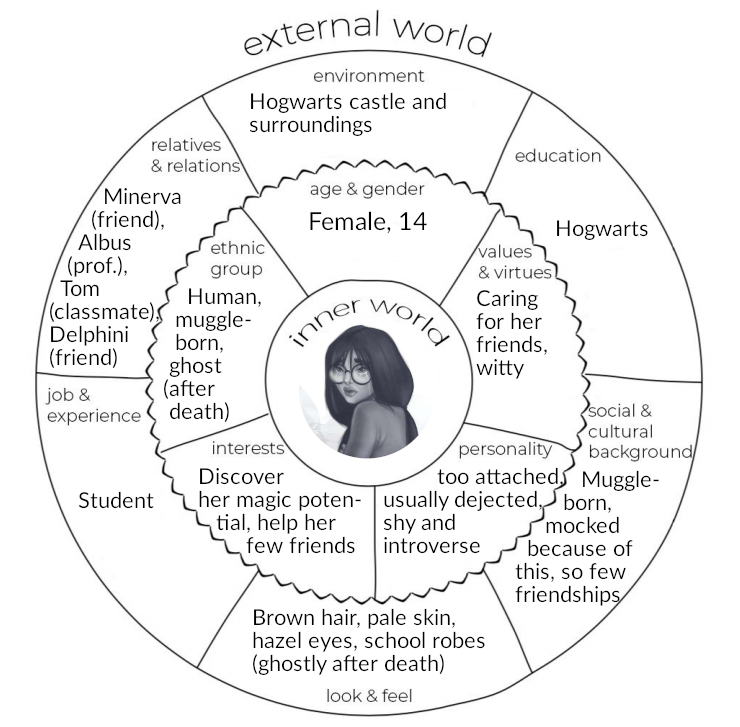
\includegraphics[max width=\textwidth]{../Pictures/Characters/Circumplexes/Myrtle_circumplex.png} 
\captionsetup{labelformat=empty}
\caption{Circumplex}
\end{figure}

\begin{figure}[H]
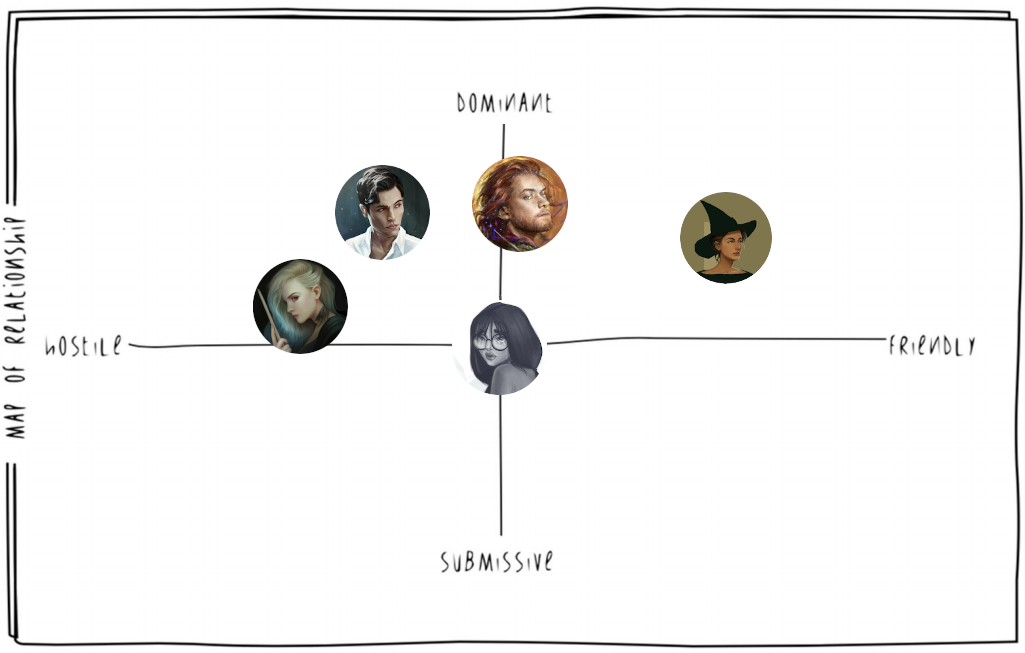
\includegraphics[max width=\textwidth]{../Pictures/Characters/Relationship_maps/Myrtle_relmap.png} 
\captionsetup{labelformat=empty}
\caption{Map of relationships}
\end{figure}


\clearpage